\section{ОТРИМАНІ РЕЗУЛЬТАТИ}

У програмному продукті використовуюються методи математичної лінгвістики,
тобто тієї галузі лінгвістики,
що займається вивченням структури природних мов, для виведення та встановлення
певних правил та мовних законів. Завдяки цьому ми можемо аналізувати збережені дані.

Оскільки архітектура програми є досить гнучкою, можна обирати будь-які
параметри для порівняння, для будь-якою мови корпусу текстів Universal
Dependencies.

\subsection{Корпус української мови}
Завдяки кінцевому програмному продукту було проаналізовано 7060 речень 
та, загалом, 122000 токенів, які мають синтаксовий шар.
Для аналізу використовувалися різні тексти, для того, щоб охопити максимальну
пвдмножину всієї мови: статті, новини, дописи, підручники, листування, казки, худпроза — і сучасні, і класичні \cite{bib12}.

Результатом аналізу корпусу української мови стали наступні законормрності,
які відображені у графіках.

На рисунку \ref{img:uk_upos} проілюстровано графік частот універсальних
частин мови, тобто upos, де видно, що у корпусі всього 17 унікальних
частин мови, де найпопулярнішою є іменник, який зустрічається в різних
місцях майже 10000 разів.

\begin{figure}[ht]
  \begin{center}
    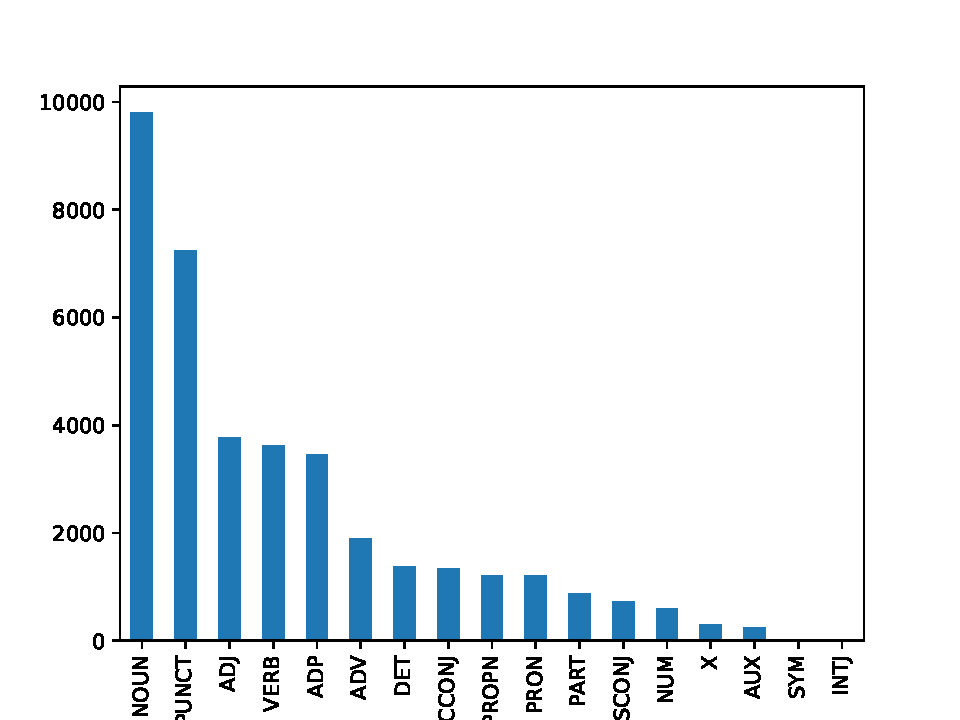
\includegraphics[width=\linewidth]{chart_uk_upos.pdf}
  \end{center}
  \caption{Графік частот універсальних частин мови}
  \label{img:uk_upos}
\end{figure}

\newpage
Порівнявши такий розподіл із законом Зіпфа, ми можемо зрозуміти, що
універсальні частини мови йому не підлягають.

На відміну від універсальних частин мови, порівнявши сигнатуру, де за основу
взяті і універсальна частина мови і її синтаксичне відношення, отримаємо
розподіл, який майже точно накладається на розподіл Зіпфа, рисунок
\ref{img:uk_deprel_upos}. Також на цьому рисунку можемо побачити, що 
всього таких сигнатур у корпусі 37722, при чому унікальних
тільки 178.

\begin{figure}[ht]
  \begin{center}
    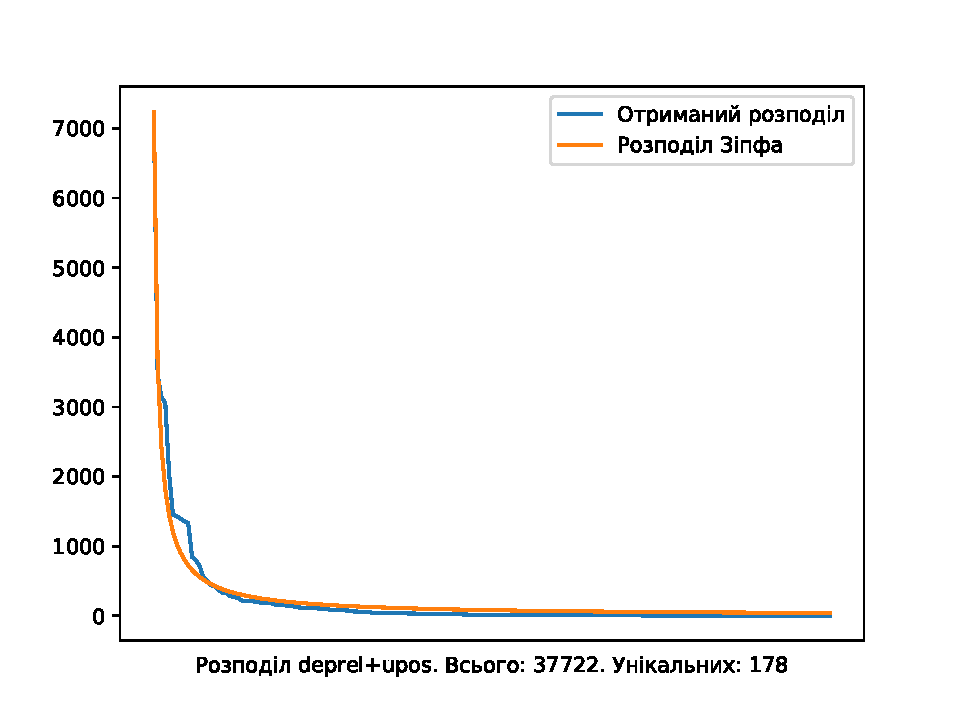
\includegraphics[width=\linewidth]{chart_uk_deprel_upos.pdf}
  \end{center}
  \caption{Розподіл частин мови та універсального відношенння}
  \label{img:uk_deprel_upos}
\end{figure}

\newpage

\begin{multicols}{2}
\begin{figure}[H]
  \begin{center}
    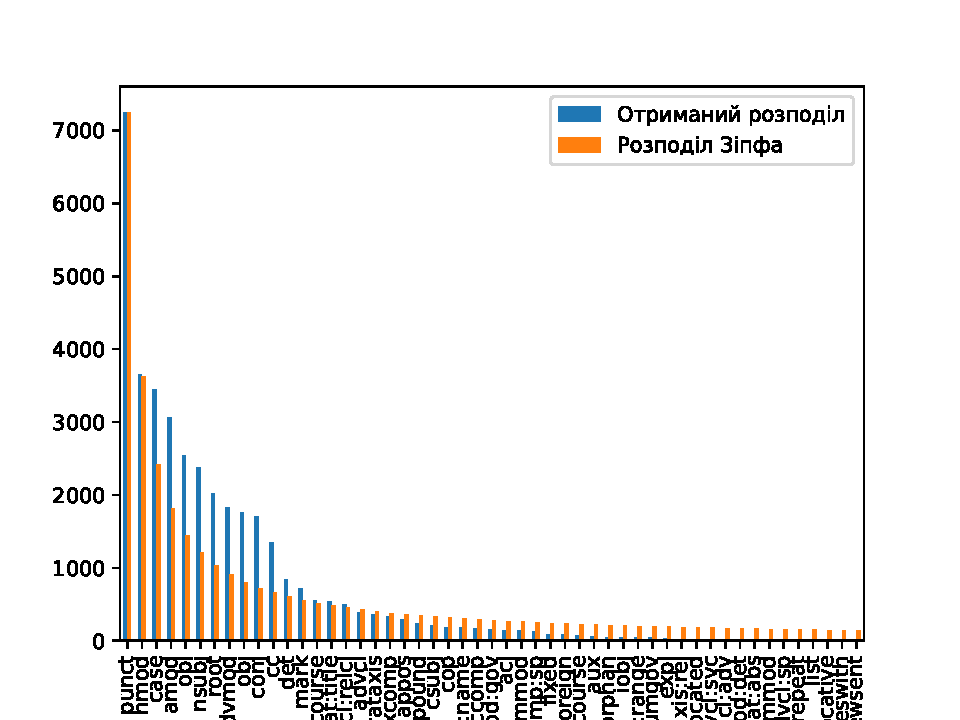
\includegraphics[width=\linewidth]{chart_uk_deprel.pdf}
  \end{center}
  \caption{Розподіл універсальних відношенннь}
  \label{img:uk0}
\end{figure}

\begin{figure}[H]
  \begin{center}
    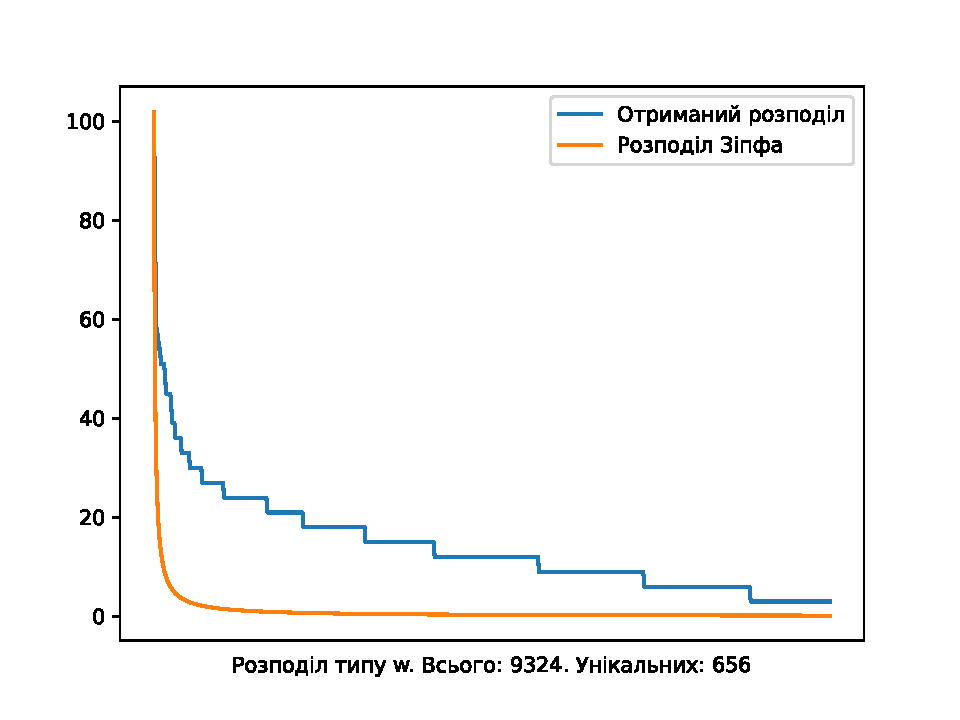
\includegraphics[width=\linewidth]{chart_uk_type_w.pdf}
  \end{center}
  \caption{Розподіл піддерев токенів, що ростуть вшир}
  \label{img:uk3}
\end{figure}

\begin{figure}[H]
  \begin{center}
    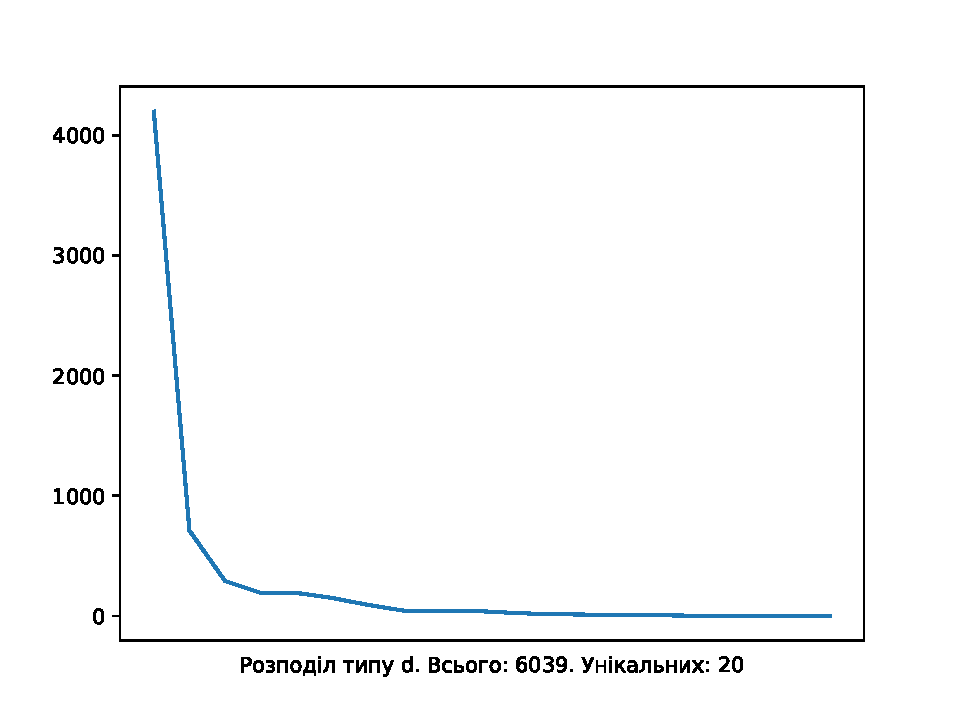
\includegraphics[width=\linewidth]{chart_uk_type_d.pdf}
  \end{center}
  \caption{Розподіл піддерев токенів, що ростуть вглиб}
  \label{img:uk4}
\end{figure}

\begin{figure}[H]
  \begin{center}
    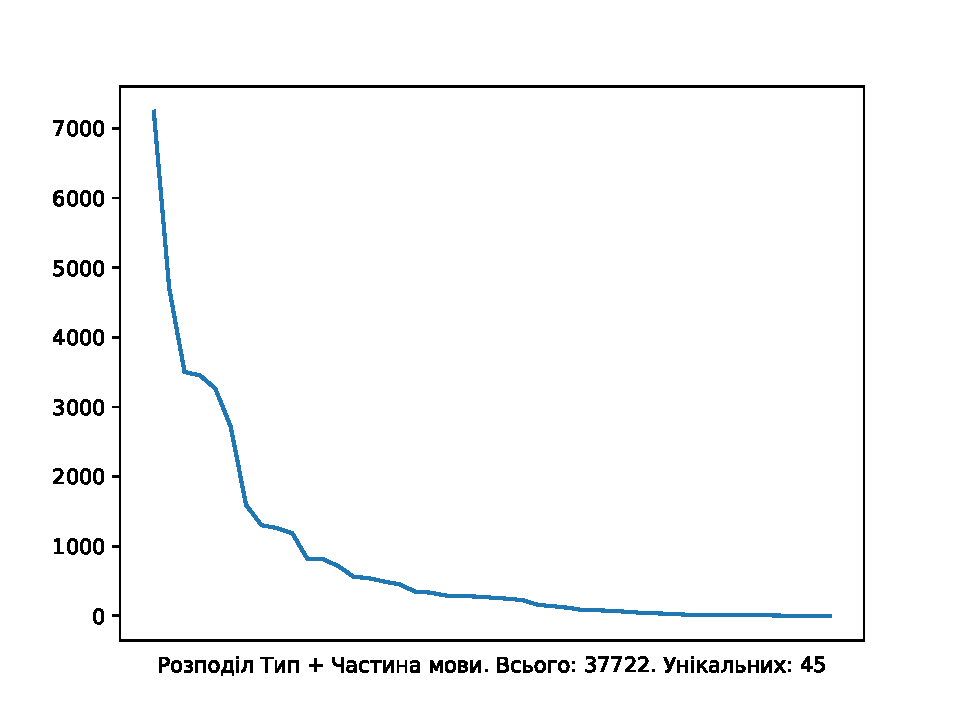
\includegraphics[width=\linewidth]{chart_uk_type_upos.pdf}
  \end{center}
  \caption{Розподіл типу та універсальної частинин мови}
  \label{img:uk5}
\end{figure}

\begin{figure}[H]
  \begin{center}
    \includegraphics[width=\linewidth]{chart_uk_sent_d_w_n.pdf}
  \end{center}
  \caption{Розподіл сигнатур речень}
  \label{img:uk6}
\end{figure}
\end{multicols}


some text

\subsection{Корпус іспанської мови}
Проаналізувавши корпус іспаномовних текстів, який щонайменше у 8 разів
більший за корпус україномовних текстів, отримаємо:

\begin{multicols}{2}
\begin{figure}[H]
  \begin{center}
    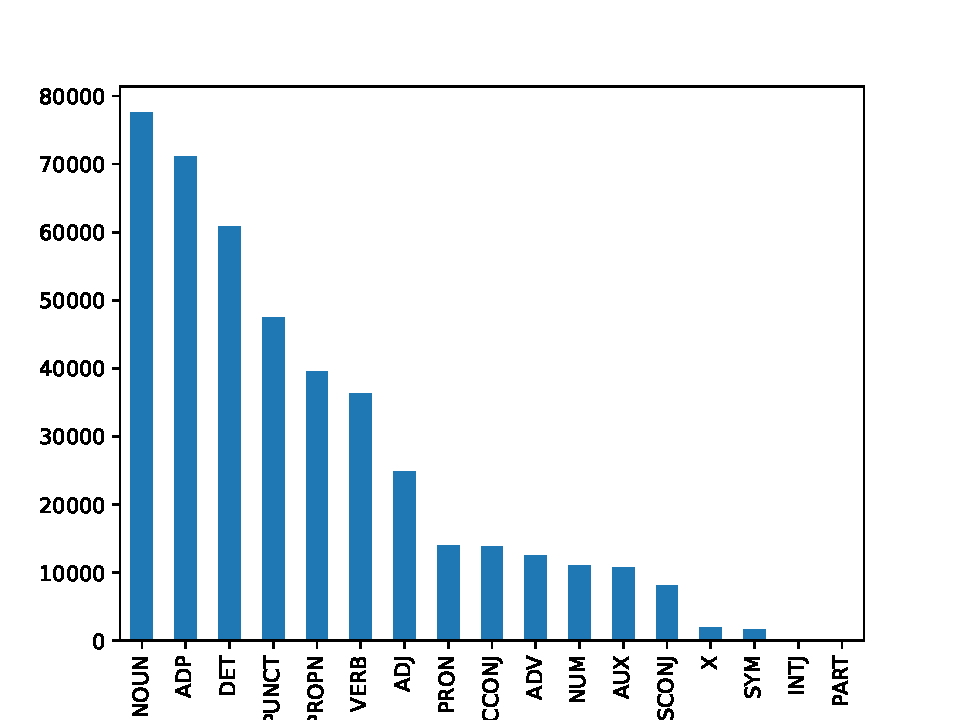
\includegraphics[width=\linewidth]{chart_es_upos.pdf}
  \end{center}
  \caption{Графік частот універсальних частин мови}
  \label{img:es_upos}
\end{figure}

\begin{figure}[H]
  \begin{center}
    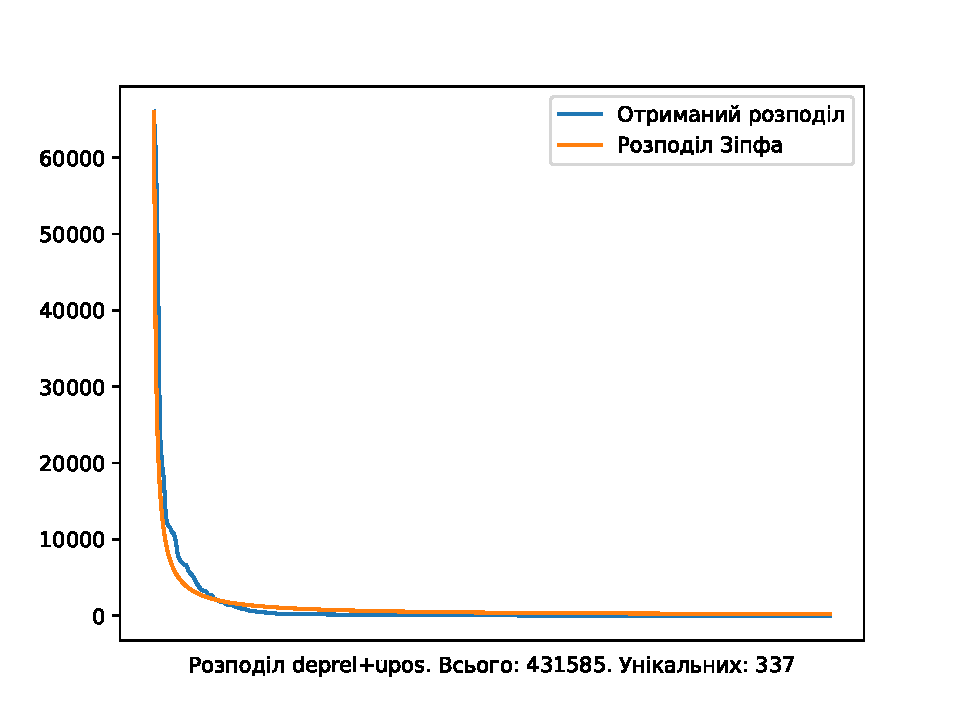
\includegraphics[width=\linewidth]{chart_es_deprel_upos.pdf}
  \end{center}
  \caption{Розподіл частин мови та універсального відношенння}
  \label{img:es_deprel_upos}
\end{figure}

\begin{figure}[H]
  \begin{center}
    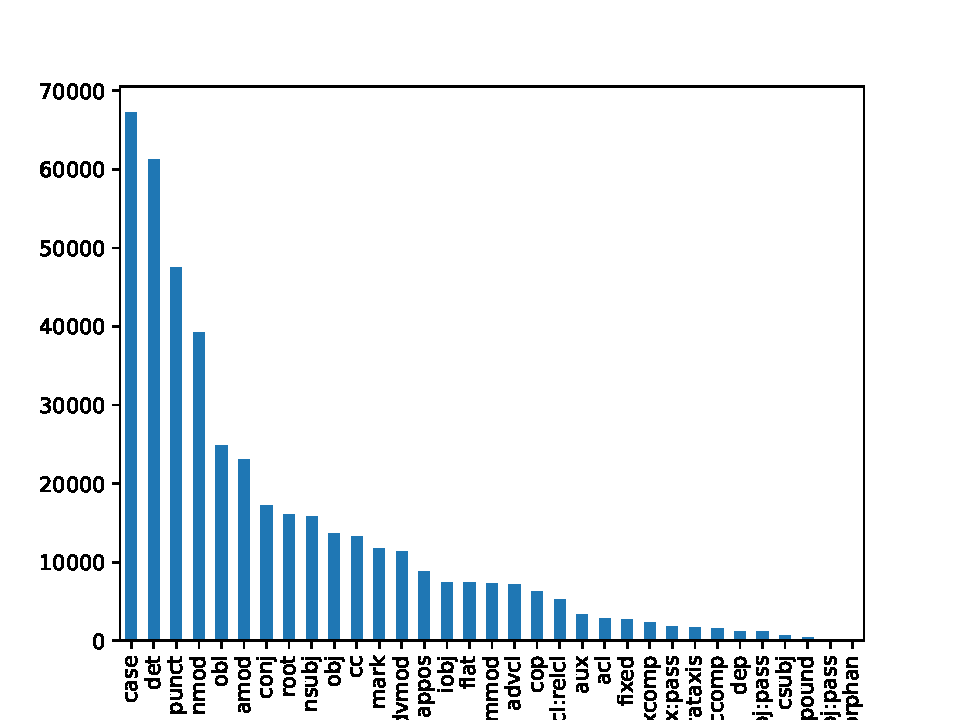
\includegraphics[width=\linewidth]{chart_es_deprel.pdf}
  \end{center}
  \caption{Розподіл універсальних відношенннь}
  \label{img:es0}
\end{figure}

\begin{figure}[H]
  \begin{center}
    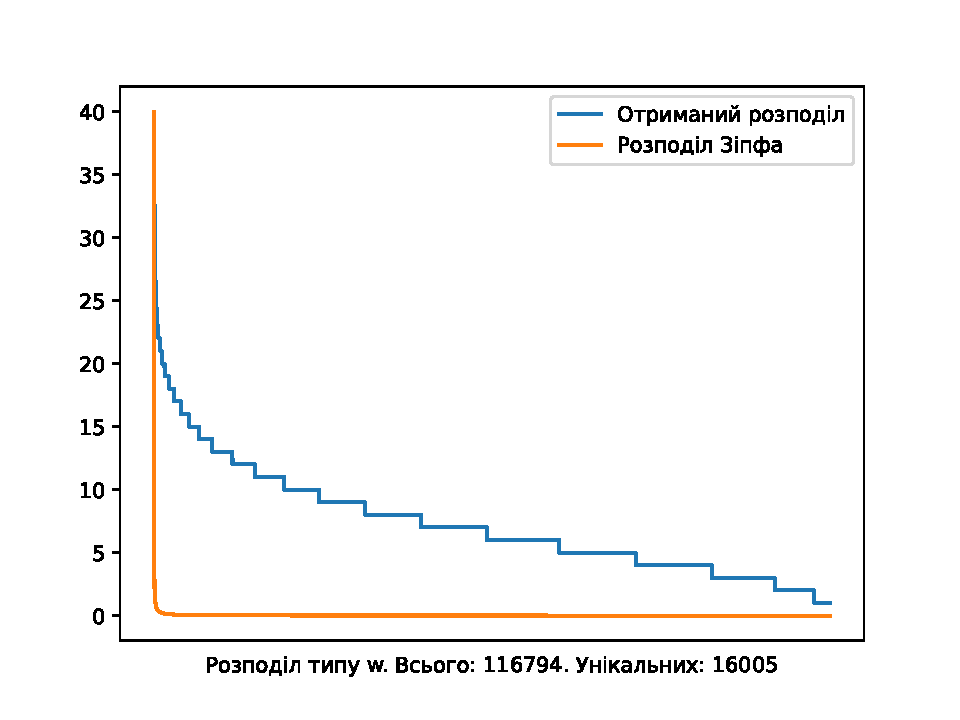
\includegraphics[width=\linewidth]{chart_es_type_w.pdf}
  \end{center}
  \caption{Розподіл піддерев токенів, що ростуть вшир}
  \label{img:es3}
\end{figure}

\begin{figure}[H]
  \begin{center}
    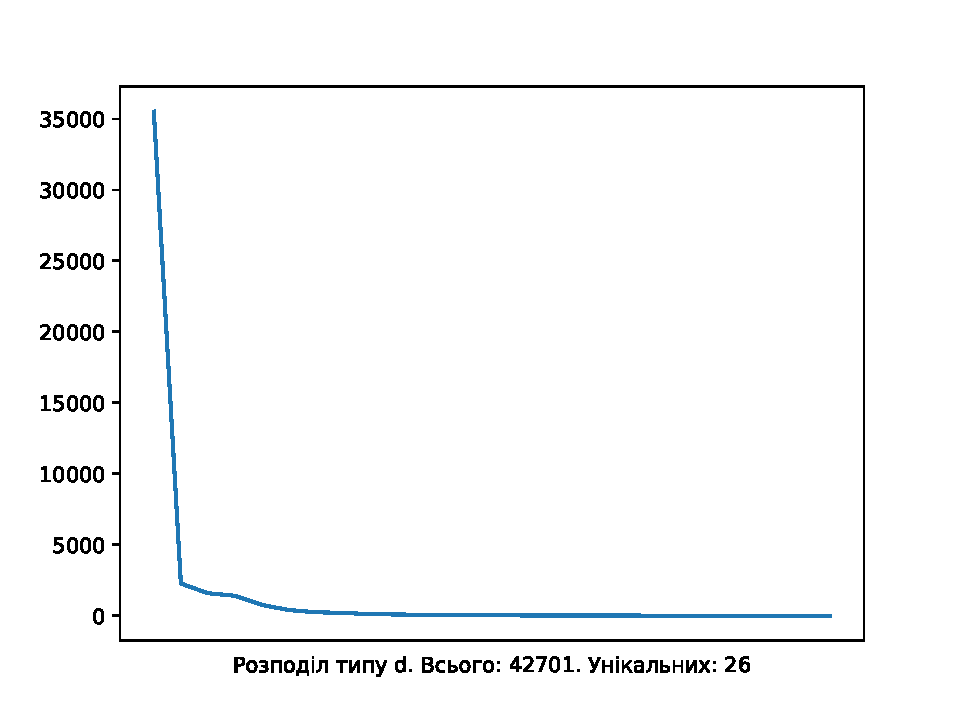
\includegraphics[width=\linewidth]{chart_es_type_d.pdf}
  \end{center}
  \caption{Розподіл піддерев токенів, що ростуть вглиб}
  \label{img:es4}
\end{figure}

\begin{figure}[H]
  \begin{center}
    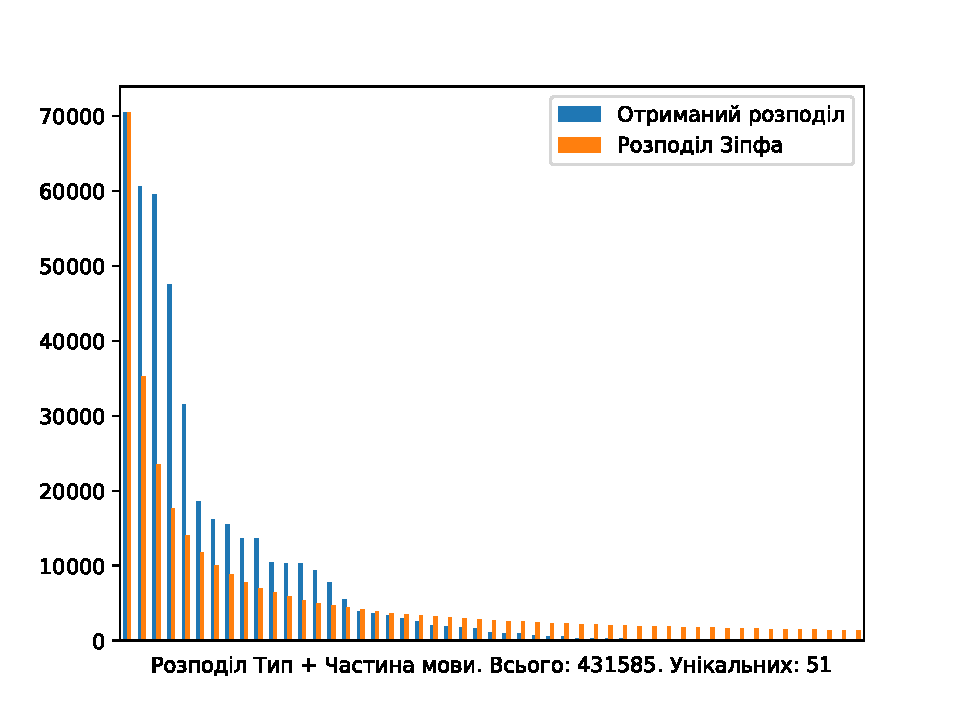
\includegraphics[width=\linewidth]{chart_es_type_upos.pdf}
  \end{center}
  \caption{Розподіл типу та універсальної частинин мови}
  \label{img:es5}
\end{figure}

\begin{figure}[H]
  \begin{center}
    \includegraphics[width=\linewidth]{article/images/chart_uk_sent_d_w_n.pdf}
  \end{center}
  \caption{Розподіл сигнатур речень}
  \label{img:es6}
\end{figure}
\end{multicols}

\subsection{Висновок}
Проаналізувавши отримані графіки, ми можемо дійти до висновку, що
тренди, які спостерігаються в україномовному корпусі майже так само
прослідковуються в іспаномовному корпусі, що підтверджує зазначену мету UD.